% =====================================================================
%  Người A -- Task 1: Khai thác và đặc tả yêu cầu
%  Nguồn: docs/requirements/context-and-scope.md, srs.md, use-case-uc01.md
%  Ngân sách: ~4,5 trang
% =====================================================================
\section{Task 1 -- Khai thác và đặc tả yêu cầu}

\subsection{Task 1.1 -- Bối cảnh, stakeholder và phạm vi}

\paragraph{Vấn đề nghiệp vụ.}
% TODO(A): 3-4 câu: quán cà phê nhỏ bán qua chat/giấy, sai sót giá và tồn kho,
% khách chờ lâu, không có dữ liệu bán hàng. BrewLite số hoá luồng đặt món.

\paragraph{Stakeholder.}
% TODO(A): bảng 6 dòng: Khách hàng, Nhân viên quầy (Barista), Quản lý cửa hàng,
% Giảng viên/khách nghiệm thu, Nhóm phát triển, Đơn vị thanh toán (ZaloPay Sandbox).
\begin{table}[H]
\centering\small
\caption{Stakeholder và kỳ vọng}
\label{tabA:stakeholder}
\begin{tabularx}{\textwidth}{@{}c l X@{}}
\toprule
\textbf{Mã} & \textbf{Stakeholder} & \textbf{Vai trò và kỳ vọng} \\
\midrule
% TODO(A)
\bottomrule
\end{tabularx}
\end{table}

\paragraph{Phạm vi.}
% TODO(A): 3 khối: In-scope MVP / Mở rộng / Out-of-scope.
% MVP: menu, chi tiết + size/topping, giỏ, auth JWT, đặt đơn, ZaloPay sandbox,
%      lịch sử + trạng thái đơn, quản trị kho/công thức/đơn/đối soát.
% Out: giao hàng, đa chi nhánh, hoá đơn điện tử, app native, thanh toán tiền thật.

\paragraph{Giả định, ràng buộc và rủi ro.}
% TODO(A): bảng rủi ro: (1) Render free ngủ -> cold start; (2) callback ZaloPay không tới
% -> polling/sync; (3) tranh chấp tồn kho -> transaction + optimistic lock;
% (4) secret lộ -> env + .gitignore; (5) thành viên trễ -> chia theo module.
\begin{table}[H]
\centering\small
\caption{Rủi ro ban đầu và biện pháp giảm thiểu}
\label{tabA:risk}
\begin{tabularx}{\textwidth}{@{}c l X@{}}
\toprule
\textbf{Mã} & \textbf{Rủi ro} & \textbf{Biện pháp} \\
\midrule
% TODO(A)
\bottomrule
\end{tabularx}
\end{table}

\subsection{Task 1.2 -- Yêu cầu chức năng và phi chức năng}

% TODO(A): 1 câu dẫn: 12 FR, 9 NFR, mức MoSCoW, mỗi yêu cầu có AC kiểm chứng được.
% Bảng FR lấy nguyên từ docs/requirements/srs.md mục 1 (đã có MoSCoW + AC).
\begin{table}[H]
\centering\footnotesize
\caption{Yêu cầu chức năng (rút gọn)}
\label{tabA:fr}
\begin{tabularx}{\textwidth}{@{}p{1.1cm} p{3.2cm} c X@{}}
\toprule
\textbf{Mã} & \textbf{Chức năng} & \textbf{MoSCoW} & \textbf{Tiêu chí chấp nhận} \\
\midrule
% TODO(A): 12 dòng FR-01..FR-12
\bottomrule
\end{tabularx}
\end{table}

\begin{table}[H]
\centering\footnotesize
\caption{Yêu cầu phi chức năng}
\label{tabA:nfr}
\begin{tabularx}{\textwidth}{@{}p{1.2cm} p{2.8cm} c X@{}}
\toprule
\textbf{Mã} & \textbf{Thuộc tính} & \textbf{MoSCoW} & \textbf{Tiêu chí chấp nhận} \\
\midrule
% TODO(A): 9 dòng NFR-01..NFR-09
\bottomrule
\end{tabularx}
\end{table}

\paragraph{Sơ đồ use-case tổng quát.}
% TODO(A): chèn hình + 3-4 câu giải thích 8 nhóm chức năng.
\begin{figure}[H]
\centering
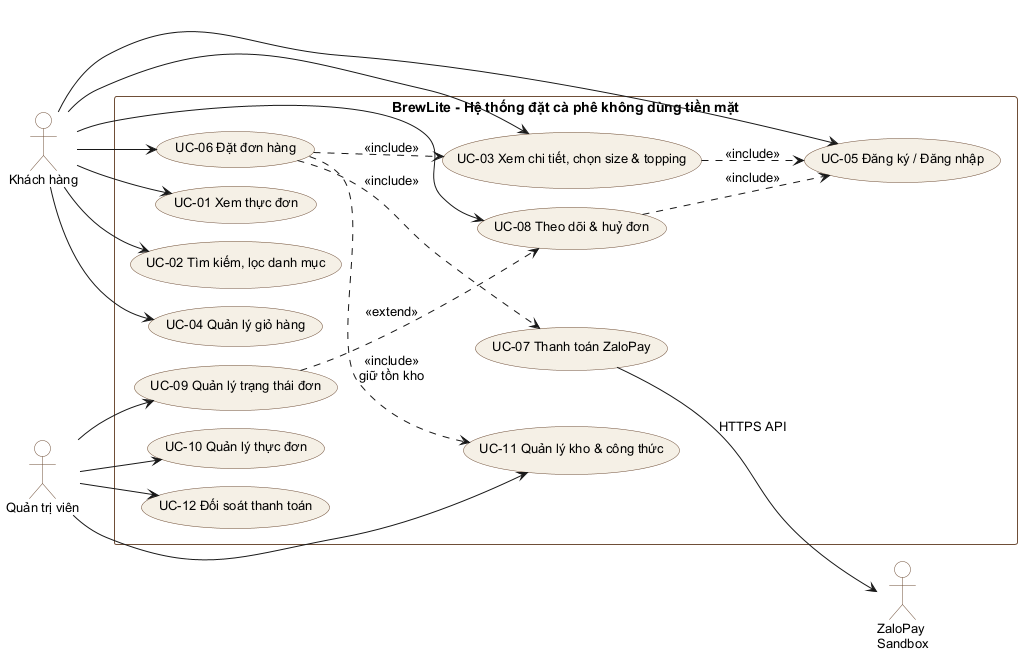
\includegraphics[width=0.82\textwidth]{../figures/diagrams/BrewLite-UseCase-Overall.png}
\caption{Sơ đồ use-case tổng quát của BrewLite}
\label{figA:usecase-overall}
\end{figure}

\subsection{Task 1.3 -- Đặc tả use-case trọng tâm: đặt và thanh toán đơn hàng}

% TODO(A): UC-01, actor chính Khách hàng, actor phụ NestJS/PostgreSQL/ZaloPay.
% Nguồn docs/requirements/use-case-uc01.md hiện chỉ mô tả TẠO ĐƠN:
%   -> BỔ SUNG bước thanh toán (FR-05, FR-08): tạo giao dịch, alt thành công/thất bại, retry.
% Bảng thông tin cơ bản: ID, tên, actor, trigger, pre-condition, post-condition.
\begin{table}[H]
\centering\small
\caption{Thông tin cơ bản UC-01}
\label{tabA:uc01}
\begin{tabularx}{\textwidth}{@{}p{3.2cm} X@{}}
\toprule
\textbf{Thuộc tính} & \textbf{Nội dung} \\
\midrule
% TODO(A): ID, Tên, Actor chính, Actor phụ, Trigger, Tiền điều kiện, Hậu điều kiện
\bottomrule
\end{tabularx}
\end{table}

\paragraph{Luồng chính.}
% TODO(A): bảng 12-14 bước, gộp tạo đơn + thanh toán. Cột: Bước | Actor | Hành động.
\begin{table}[H]
\centering\small
\caption{Luồng chính UC-01}
\label{tabA:uc01-main}
\begin{tabularx}{\textwidth}{@{}c l X@{}}
\toprule
\textbf{Bước} & \textbf{Actor} & \textbf{Hành động} \\
\midrule
% TODO(A)
\bottomrule
\end{tabularx}
\end{table}

\paragraph{Luồng thay thế và ngoại lệ.}
% TODO(A): bảng: hết hàng (FR-09), chưa đăng nhập (FR-04), payment fail (FR-05),
% trùng Idempotency-Key (FR-08), đơn quá hạn (FR-07). Cột: Mã | Tại bước | Xử lý | Kết quả | FR.
\begin{table}[H]
\centering\small
\caption{Luồng thay thế và ngoại lệ UC-01}
\label{tabA:uc01-alt}
\begin{tabularx}{\textwidth}{@{}c c X X@{}}
\toprule
\textbf{Mã} & \textbf{Bước} & \textbf{Điều kiện và xử lý} & \textbf{Liên kết FR} \\
\midrule
% TODO(A)
\bottomrule
\end{tabularx}
\end{table}
